\documentclass{article}
\usepackage[UTF8]{ctex}
\usepackage{amsmath,mathtools}
\usepackage{color}
\usepackage{float}
\usepackage{esint}%积分符号
\newcommand{\point}[1]{$\color{blue}{\text{#1}}$}
\setlength{\parindent}{0pt}%不缩进

\title{普物复习}
\author{191220090 沈天杰}
\begin{document}
    \maketitle
    {\centering\tableofcontents}
    \section{静止电荷的电场}
    \noindent基本物理量: 电荷\quad电场强度\quad电势\footnote{电势梯度与场强}\\
    基本定律:电荷守恒定律,库仑定律,场强叠加原理,高斯定律,安培环路定理
    \subsection{电场、电荷\quad库仑定律}
    \[
        \vec{F_{12}}=\frac{1}{4\pi\epsilon_0}\frac{q_1q_2}{r_{12}^2}(\frac{\vec{r_{12}}}{r_{12}})    
    \]
    其中$\frac{1}{4\pi\epsilon_0}\approx 8.988\times 10^9 N\cdot m^2\cdot C^{-2}$\\
    \point{考题}:库仑定律和力的叠加原理
    \subsection{电场\quad电场强度}
    \noindent电场强度是随位置而变的矢量场
    \[
      \vec{E}=\frac{\vec{F}}{q_0}=\frac{Q}{4\pi\epsilon_0r^2} \hat{r} \quad \textbf{点电荷的场强} 
    \]
    场强叠加原理 离散与连续。\\\\
    \point{考题1}:两电荷连线的中垂面上任意一点P的电场强度\\
    电偶极子(或称电偶极矩):$\vec{p}=q\vec{l}$\\
    电偶极子在其延长线上远场点电场强度$E=\frac{p_e}{2\pi\epsilon_0r^3}$
    注意\;1)\;l很小(相对于r) 2)\;方向从负电荷指向正电荷。\\
    点P的电场强度方向与电偶极子相反。电偶极子的电场强度是立方衰减的。\\
    \point{考题2}:无限长均匀带电细棒中垂面上的场强分布\\
    \[
        E_y=\frac{1}{4\pi\epsilon_0}\frac{2\lambda}{a}
    \]
    其中a为待测点到细棒距离。\\
    \point{考题3}:带电圆环轴线上的电场强度。P点离环心的距离为x。\par
    \[
        \vec{E}=\frac{qx}{4\pi\epsilon_0(R^2+x^2)^{3/2}}\hat{i}  
    \]
    当$x\to \infty$电场强度时等同于点电荷\\
    \point{考题4}:带电圆盘轴线上的电场强度。圆盘半径为R,面密度为$\sigma$:\\
    \[
    E_x=\frac{\sigma}{2\epsilon_0}(1-\frac{1}{\sqrt{1+R^2/x^2}})    
    \]
    1)R$\ll$x \; 点电荷 \\
    2)R$\gg$x \; $E_x=\frac{\sigma}{2\epsilon_0}$ \; 相当于无限大板。匀强电场,和距离无关。\\
    \point{考题5}\textbf{无限大面和无限长线上电荷的综合运用(重点)}
    \begin{figure}[H]
        \centering
        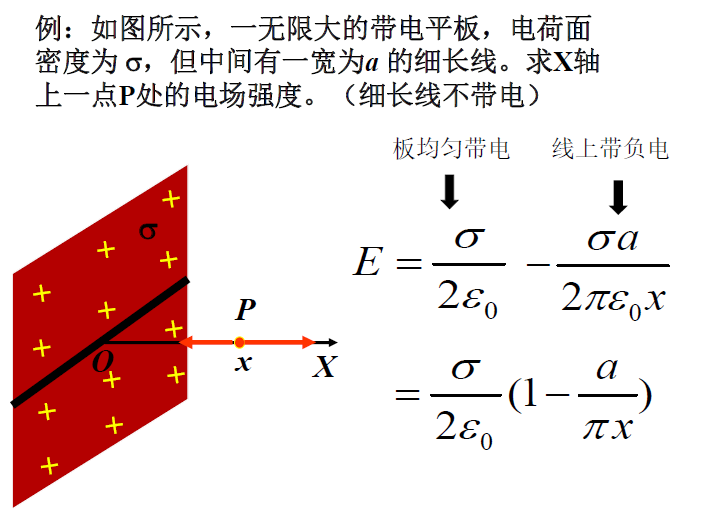
\includegraphics[width=.95\textwidth]{figure/inf.png}
    \end{figure}
    \point{总结}:计算场强分布的三种办法:1。库仑定律+场强叠加原理2。电荷对称性分布:高斯定理3。电势梯度
    \subsection{电场线}
    \noindent电场线:电场线上每一点的切线方向都与该点的场强E方向一致;在与电场强度垂直的单位面积中,所穿过的电场线根数与该处的场强大小成正比。
    \[
    dN\sim EdS \quad E\sim dN/dS    
    \]
    即:场强正比于与其垂直的单位面积内穿过的电力线根数。\\
    性质:
    \begin{enumerate}
        \item 起自正电荷(或无限远),终止于负电荷(或伸向无穷远),但不会在没有电荷的地方中断。(高斯定理)
        \item 静电场的电场线不能形成闭合曲线,无旋场。(环路定理)
        \item 电力线越密的地方,场强越大;电力线越疏的地方,场强越小。
        \item 任何两条电场线不会相交。
        \item 电场线的方向反映正电荷在各点的受力方向,但电场线不是正电荷的运动轨迹。
    \end{enumerate}
    借助电场线,引入\point{电场强度通量}$\psi_E=ES$\\
    对整个曲面积分可求得面积为S的任意曲面E通量
    \[
    \psi_E=\iint_S Ecos\theta dS =\iint_S E\cdot dS
    \]
    S为闭合曲面时,曲面内部穿出E通量为正,外部穿入E通量为负。
    \[
    \psi_E=\oiint_S Ecos\theta dS =\oiint_S E\cdot dS
    \]
    \subsection{高斯定理}
    \noindent以点电荷q为球心的球面的E通量都等于$q/\epsilon_0$\\
    通过电场中任一闭合曲面的总电通量,等于该曲面内包围的所有电荷电量的代数和除以$\epsilon_0$,而与闭合面外的电荷无关。
    \[
      \oint_S \vec{E}\cdot d\vec{S}=\frac{1}{\epsilon_0}\sum_{\text{S内}} q_i  
    \]
    虽然高斯面上的电通量只和内部电荷量有关,但不能说:高斯面上电场只是由内部电荷决定的。高斯面上的电场是由全空间电荷共同决定的。\\
    \point{高斯定理的应用}\\
    适用情况:通常是具有某种对称性的电场--轴对称、球对称、均匀场等。\\
    应用方法:先作对称性分析。\\
    静电场是有源场.
    \subsection{静电场的环路定理、电势(电位)}
    \subsubsection{环路定理}
    场强环路定理——\point{静电场}中,沿任一闭合路径场强的环流等于零.
    \[
      \oint_L \vec{E}\cdot d\vec{l}=0  
    \]
    物理含义:静电场是保守力场(可定义电势能和电势);微分形式即无旋场。
    \subsubsection{电势(电位)}
    电场中a点的电势是描写电势能\footnote{电荷$q_0$在电场中某点a具有的电势能\textbf{等于}电场力将此电荷从参考点移至a点电场力所作的功的负值。}的物理量。
    \[
    V_a=w_a/q_0=-\int_{\text{参}}^a \vec{E}\cdot d\vec{l}    
    \]
    特殊的\;单个点电荷电势为$\frac{q}{4\pi\epsilon_0r}$\\
    电势叠加原理:点电荷电场中一点的电势,等于每一点电荷单独在这一点所产生的电势的\point{代数和}。\\
    \point{考题}:带电q半径R球壳
    \begin{enumerate}
        \item 球壳场强
        \begin{equation*}
            \vec{E}=
            \begin{cases}
                0 & (0\leq r \textless R)\\
                \frac{q}{4\pi\epsilon_0r^2}\hat{r}&(R\leq r \textless \infty)
            \end{cases}
        \end{equation*}
        \item 球壳电势
        \begin{equation*}
            V(r)=
            \begin{cases}
                \frac{q}{4\pi\epsilon_0R} & (0\leq r \textless R)\\
                \frac{q}{4\pi\epsilon_0r} & (R\leq r \textless \infty)
            \end{cases}
        \end{equation*}
    
    
    \end{enumerate}
    计算电势的方法:\;1。先计算场强,然后积分计算\;2。叠加原理。
    \subsection{等势面\quad电场强度与电势梯度的关系}
    等势面性质:
    \begin{itemize}
        \item 等势面与电力线处处正交。
        \item 等势面密集的地方场强大,稀疏的地方场强小。
    \end{itemize}
    由梯度的定义,有$dV=\nabla V \cdot d\vec{l}$\\
    场强方向即梯度逆方向,即电势下降最快的方向。
    \[
      \vec{E}=-\nabla V    
    \]
    其中$\vec{\nabla} \equiv \vec{i}\frac{\partial}{\partial x}+\vec{j}\frac{\partial}{\partial y}+\vec{k}\frac{\partial}{\partial z}$
    \subsection{静电场中的导体}
    \subsection{电容器与电容}
    \subsection{静电场的能量}
    \section{恒定电流及其磁场}
    \section{电磁感应、麦克斯韦方程组}
\end{document}